\documentclass[aspectratio=169,11pt]{beamer}
\usepackage[T1]{fontenc}
\usepackage{lmodern}
\usepackage{listings,booktabs,tikz,graphicx}
\usetikzlibrary{arrows.meta,positioning,fit}
\definecolor{navy}{HTML}{18344B}
\definecolor{teal}{HTML}{087F8C}
\definecolor{paper}{HTML}{F1F5F8}
\setbeamercolor{normal text}{fg=navy,bg=white}
\setbeamercolor{frametitle}{fg=navy}
\setbeamercolor{structure}{fg=teal}
\setbeamercolor{block title}{fg=white,bg=teal}
\setbeamercolor{block body}{bg=paper}
\setbeamertemplate{navigation symbols}{}
\setbeamercolor{footline}{fg=navy,bg=white}
\setbeamertemplate{footline}{%
  \begin{beamercolorbox}[wd=\paperwidth,ht=3.5ex,dp=1.5ex,rightskip=5mm]{footline}%
    \hfill\scriptsize Agentic AI for Games\quad
    \insertframenumber\,/\,\inserttotalframenumber
  \end{beamercolorbox}}
\setbeamertemplate{itemize items}[circle]
\setbeamersize{text margin left=9mm,text margin right=9mm}
\lstset{language=Python,basicstyle=\ttfamily\small,keywordstyle=\color{teal}\bfseries,
 stringstyle=\color{navy},commentstyle=\color{gray},backgroundcolor=\color{paper},
 showstringspaces=false,columns=fullflexible,keepspaces=true,breaklines=true,
 frame=none,xleftmargin=2mm,xrightmargin=2mm,aboveskip=2mm,belowskip=2mm}
\tikzset{box/.style={draw=teal,fill=paper,rounded corners=2pt,minimum height=12mm,
 text width=30mm,align=center,font=\small,inner sep=3mm},arr/.style={-{Latex[length=2mm]},thick,draw=navy}}
\newcommand{\src}[1]{\par\vspace{1mm}{\tiny\color{gray}\texttt{\detokenize{#1}}}\par}
\newcommand{\takeaway}[1]{\vspace{3mm}\begin{block}{}#1\end{block}}
\title{Agentic AI for Games}
\subtitle{From language models to tools, ReAct and MCP}
\author{Simon Lucas}
\date{Tutorial snapshot: 14 September 2026}
\begin{document}
\begin{frame}
\titlepage
\centering\small Python examples: exact counting $\rightarrow$ search $\rightarrow$ gameplay, PCG
\end{frame}

\begin{frame}{Why give an LLM tools?}
\begin{columns}[T]
\column{.48\textwidth}
\textbf{Language models are useful for}
\begin{itemize}
\item Interpreting a task and its rules.
\item Proposing actions and strategies.
\item Choosing which capability to use.
\end{itemize}
\column{.48\textwidth}
\textbf{Code supplies concrete capabilities}
\begin{itemize}
\item Exact arithmetic and counting.
\item Access to current game state.
\item Simulation, search and validation.
\end{itemize}
\end{columns}
\takeaway{Let the model choose an operation; let tested code perform it.}
\small Tools can improve reliability. Choosing the wrong tool or arguments can still fail.
\end{frame}

\begin{frame}{Start with an ordinary Python function}
\lstinputlisting{snippets/function.py}
\src{src/simple_examples/operations.py}
\begin{itemize}
\item Calling \texttt{multiply(6, 7)} returns \texttt{42}.
\item No language model or protocol is needed for this calculation.
\item The agentic step is deciding \emph{when} to call it from a language request.
\end{itemize}
\takeaway{Separate the capability from the machinery that invokes it.}
\end{frame}

\begin{frame}{ReAct: reason, act, observe, repeat}
\centering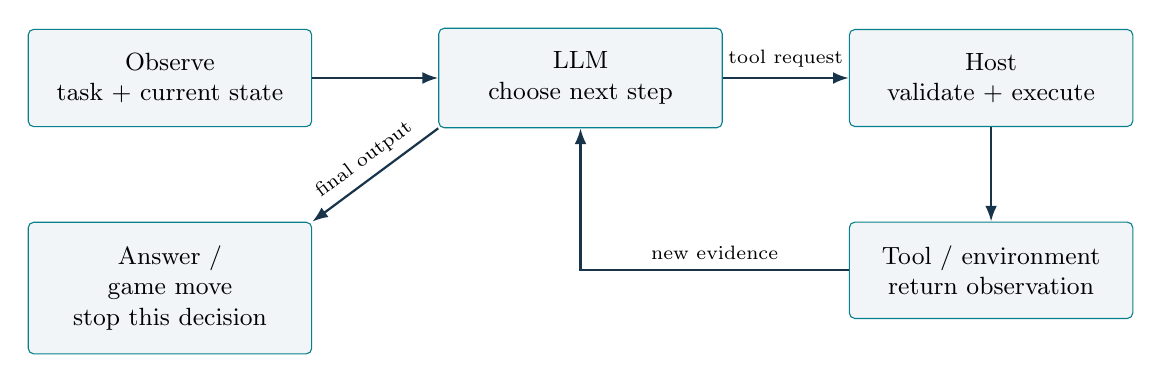
\begin{tikzpicture}[node distance=12mm and 16mm]
\node[box] (state) {Observe\\task + current state};
\node[box,right=of state] (llm) {LLM\\choose next step};
\node[box,right=of llm] (host) {Host\\validate + execute};
\node[box,below=of host] (tool) {Tool / environment\\return observation};
\node[box,below=of state] (done) {Answer / game move\\stop this decision};
\draw[arr] (state)--(llm);
\draw[arr] (llm)--node[above,font=\scriptsize]{tool request}(host);
\draw[arr] (host)--(tool);
\draw[arr] (tool.west)-|node[pos=.25,above,font=\scriptsize]{new evidence}(llm.south);
\draw[arr] (llm.south west)--node[above,sloped,font=\scriptsize]{final output}(done.north east);
\end{tikzpicture}

\par\vspace{3mm}\raggedright\small
ReAct interleaves reasoning and actions, using observations to revise the next step.
Our function-calling loop follows this pattern; it does not require a printed
``Thought:'' transcript or expose a model's private reasoning.
\src{Yao et al., ReAct, ICLR 2023. https://arxiv.org/abs/2210.03629}
\end{frame}

\begin{frame}{One concrete interaction}
\begin{enumerate}
\item \textbf{Task:} ``What is six times seven?''
\item \textbf{Model action:} request \texttt{multiply(a=6, b=7)}.
\item \textbf{Host action:} execute the tool and collect \texttt{42}.
\item \textbf{Observation:} append the result to the conversation.
\item \textbf{Model answer:} ``42.''
\end{enumerate}
\takeaway{A tool call is a structured request. The host runs the code.}
\small Stop on a final answer; bound the number of calls and handle failures.
\end{frame}

\begin{frame}{Why introduce MCP?}
\textbf{Model Context Protocol: a shared interface to capabilities.}
\begin{itemize}
\item Discover tool names, descriptions and input schemas.
\item Invoke a tool with structured arguments; receive its result.
\item Reuse a server across compatible host applications.
\end{itemize}
\takeaway{ReAct describes the loop. MCP connects the loop to tools.}
\small Direct Python calls remain sufficient inside one application. MCP adds a
reusable process/service boundary. It does not make a tool or model correct.
\end{frame}

\begin{frame}{The architecture in this repository}
\centering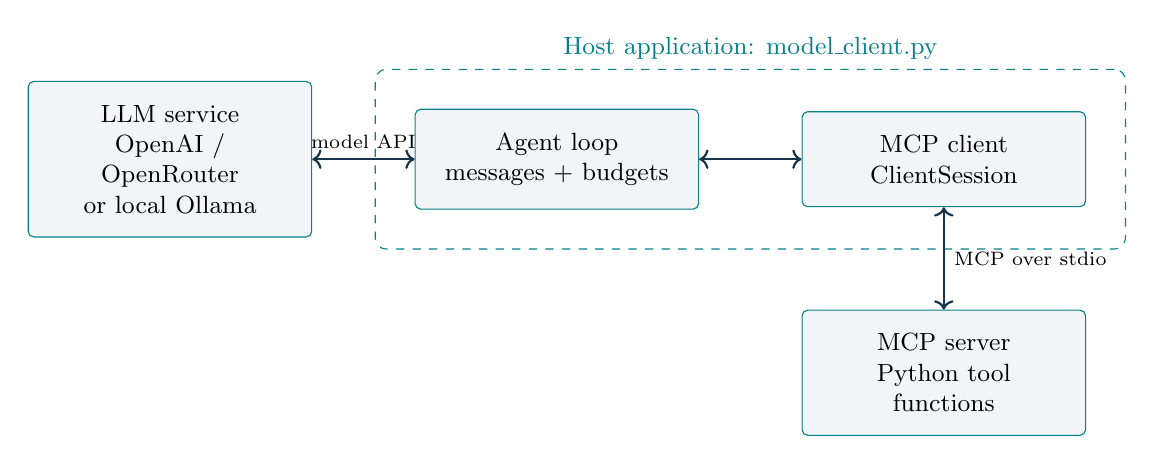
\begin{tikzpicture}[node distance=10mm and 13mm]
\node[box] (llm) {LLM service\\OpenAI / OpenRouter\\or local Ollama};
\node[box,right=of llm] (loop) {Agent loop\\messages + budgets};
\node[box,right=of loop] (client) {MCP client\\ClientSession};
\node[box,below=13mm of client] (server) {MCP server\\Python tool functions};
\node[draw=teal,dashed,rounded corners,fit=(loop)(client),inner sep=5mm,
 label={[font=\small,text=teal]above:Host application: model\_client.py}] {};
\draw[<->,thick,draw=navy] (llm)--node[above,font=\scriptsize]{model API}(loop);
\draw[<->,thick,draw=navy] (loop)--(client);
\draw[<->,thick,draw=navy] (client)--node[right,font=\scriptsize]{MCP over stdio}(server);
\end{tikzpicture}

\par\vspace{4mm}\raggedright\small
Component notation: boxes are responsibilities; the dashed boundary is the host.
The model API and the MCP connection are separate interfaces.
\src{MCP architecture, specification 2025-06-18; implemented here with the Python SDK.}
\end{frame}

\begin{frame}{Expose the function as an MCP tool}
\lstinputlisting{snippets/server.py}
\src{src/simple_examples/server.py}
\begin{itemize}
\item \texttt{@mcp.tool()} registers a callable capability.
\item Type hints describe inputs; the docstring explains its purpose.
\item The server starts with \texttt{mcp.run(transport="stdio")}.
\end{itemize}
\small With stdio, keep diagnostic output off stdout: it carries protocol messages.
\end{frame}

\begin{frame}[fragile]{Same decorator, different variable names}
\begin{lstlisting}[basicstyle=\ttfamily\footnotesize]
# simple_examples/server.py
mcp = FastMCP("beginner-arithmetic-and-strings")
@mcp.tool()
def multiply(a: float, b: float) -> float:
    ...

# griddle/search_server.py, inside create_server()
server = FastMCP("griddle-search", log_level="WARNING")
@server.tool()
def mcs_advice(rollouts_per_square: Budget = 10) -> dict:
    ...
\end{lstlisting}
\small Abbreviated repo excerpts. Both objects are \texttt{FastMCP} instances.
\par\vspace{2mm}\textbf{Register on the chosen server object; its variable name is arbitrary.}\par\vspace{2mm}
\small \texttt{@mcp.tool()} means \texttt{function = mcp.tool()(function)}.
It registers the function when this definition executes; it does not run it.
\end{frame}

\begin{frame}{MCP decorators: operation, context or template?}
\small
\begin{tabular}{p{.36\textwidth}p{.57\textwidth}}
\toprule Decorator & When to use it\\\midrule
\texttt{@mcp.tool()} & An operation: compute, search or act.\\[3mm]
\texttt{@mcp.resource(uri)} & Addressable context the application can read, such as game rules.\\[3mm]
\texttt{@mcp.prompt()} & A reusable, user-selectable prompt template; it does not call the model.\\[3mm]
\texttt{@mcp.completion()} & Suggestions for prompt/resource arguments.\\\bottomrule
\end{tabular}
\takeaway{This repository registers tools only. The host decides which to offer to the LLM.}
\small Griddle's \texttt{configure} and \texttt{set\_position} are registered tools,
but excluded from the model's allowlist. Registration is not a privacy boundary.
\end{frame}

\begin{frame}{Other decorators have different jobs}
\small
\begin{tabular}{p{.42\textwidth}p{.51\textwidth}}
\toprule Decorator & Purpose in this repository\\\midrule
\texttt{@dataclass(frozen=True, ...)} & Pydantic validation; frozen fields.\\[1mm]
\texttt{@model\_validator(...)} & Cross-field checks, e.g. unique tool names.\\[1mm]
\texttt{@asynccontextmanager} & Acquire and close clients around \texttt{async with}.\\[1mm]
\texttt{@classmethod} & Alternate constructor: \texttt{new\_game(cls, ...)}.\\[1mm]
\texttt{@staticmethod} & Class helper without implicit \texttt{self}: \texttt{\_rollout}.\\[1mm]
\texttt{@property} & Computed attribute: \texttt{match.score}.\\\bottomrule
\end{tabular}
\takeaway{These organise Python behaviour; none exposes an MCP tool.}
\small Decorators apply when definitions execute. Read the import or owning object
to understand what each one does.
\src{docs/decorators.md; src/game_agent/griddle/}
\end{frame}

\begin{frame}{Discover and call a tool without an LLM}
\lstinputlisting[basicstyle=\ttfamily\footnotesize]{snippets/discovery.py}
\src{src/simple_examples/mcp_client.py}
\takeaway{Test the protocol and tools independently before adding model behaviour.}
\end{frame}

\begin{frame}{Bridge MCP schemas to the model API}
\begin{columns}[T]
\column{.64\textwidth}
\lstinputlisting[basicstyle=\ttfamily\footnotesize]{snippets/schema.py}
\column{.32\textwidth}
\vspace{4mm}
\begin{itemize}
\item The model sees a tool's name, purpose and argument schema.
\item It does not receive the Python function body.
\item The host translates between the two interfaces.
\end{itemize}
\end{columns}
\src{src/simple_examples/model_client.py : as_model_tools}
\end{frame}

\begin{frame}{The loop: ask the model for its next step}
\lstinputlisting[basicstyle=\ttfamily\footnotesize]{snippets/request.py}
\src{src/simple_examples/model_client.py : answer (excerpt)}
\small \texttt{tool\_choice="auto"} allows either a tool request or an answer.
The eight-round bound prevents an unending loop.
\end{frame}

\begin{frame}{The loop: execute and return the observation}
\lstinputlisting[basicstyle=\ttfamily\footnotesize]{snippets/execute.py}
\src{src/simple_examples/model_client.py : answer (excerpt)}
\small The call ID links each observation to the request it answers.
\end{frame}

\begin{frame}{The same interaction as a sequence diagram}
\centering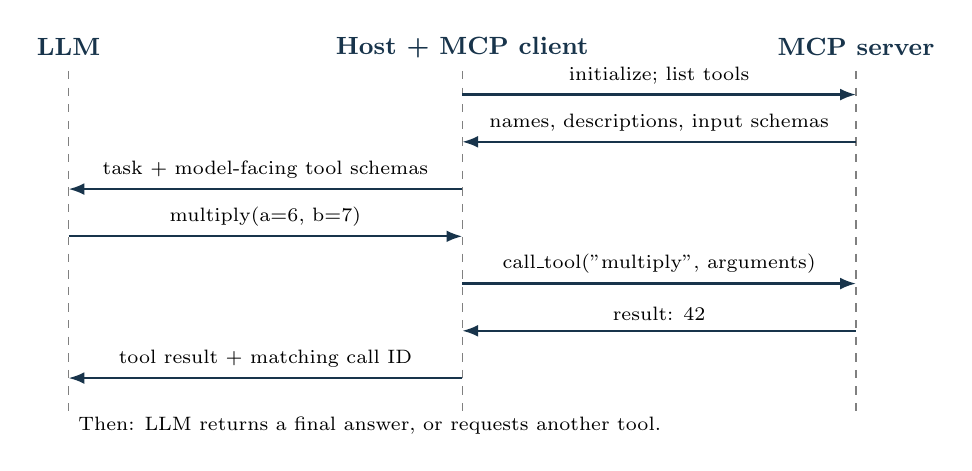
\begin{tikzpicture}[x=1cm,y=1cm]
\foreach \x/\label in {0/LLM,5/Host + MCP client,10/MCP server}{
 \node[font=\small\bfseries,text=navy] at (\x,0) {\label};
 \draw[dashed,gray] (\x,-.3)--(\x,-4.65);
}
\draw[arr] (5,-.6)--node[above,font=\scriptsize]{initialize; list tools}(10,-.6);
\draw[arr] (10,-1.2)--node[above,font=\scriptsize]{names, descriptions, input schemas}(5,-1.2);
\draw[arr] (5,-1.8)--node[above,font=\scriptsize]{task + model-facing tool schemas}(0,-1.8);
\draw[arr] (0,-2.4)--node[above,font=\scriptsize]{multiply(a=6, b=7)}(5,-2.4);
\draw[arr] (5,-3)--node[above,font=\scriptsize]{call\_tool("multiply", arguments)}(10,-3);
\draw[arr] (10,-3.6)--node[above,font=\scriptsize]{result: 42}(5,-3.6);
\draw[arr] (5,-4.2)--node[above,font=\scriptsize]{tool result + matching call ID}(0,-4.2);
\node[font=\scriptsize,anchor=west] at (0,-4.8) {Then: LLM returns a final answer, or requests another tool.};
\end{tikzpicture}

\end{frame}

\begin{frame}{From arithmetic to Griddle}
\begin{columns}[T]
\column{.57\textwidth}
\begin{itemize}
\item Place 25 sequential letters on a $5\times5$ grid.
\item Each placement is permanent; future cards are hidden.
\item Score contiguous words left-to-right and top-to-bottom.
\item Overlaps and subwords count; one-letter words do not.
\end{itemize}
\column{.39\textwidth}
\begin{tabular}{rr}
\toprule Word length & Points\\\midrule
2 & 1\\3 & 3\\4 & 7\\5 & 10\\\bottomrule
\end{tabular}
\par\vspace{5mm}\small
This implementation: 73-card deck; bundled dictionary is authoritative.
\end{columns}
\takeaway{The objective is expected final score, not just an immediate word.}
\end{frame}

\begin{frame}{Monte Carlo Search (MCS) as a tool}
\lstinputlisting[basicstyle=\ttfamily\footnotesize]{snippets/search.py}
\src{src/game_agent/griddle/search_server.py}
\small For each empty square: place the letter in a simulation, complete the game
randomly, average the final scores. Repeat $B$ times per square.
\takeaway{At 25 empty squares and $B=10$: 250 simulated completions.
These are noisy estimates, not guaranteed outcomes.}
\end{frame}

\begin{frame}{Keep advice separate from real game actions}
\centering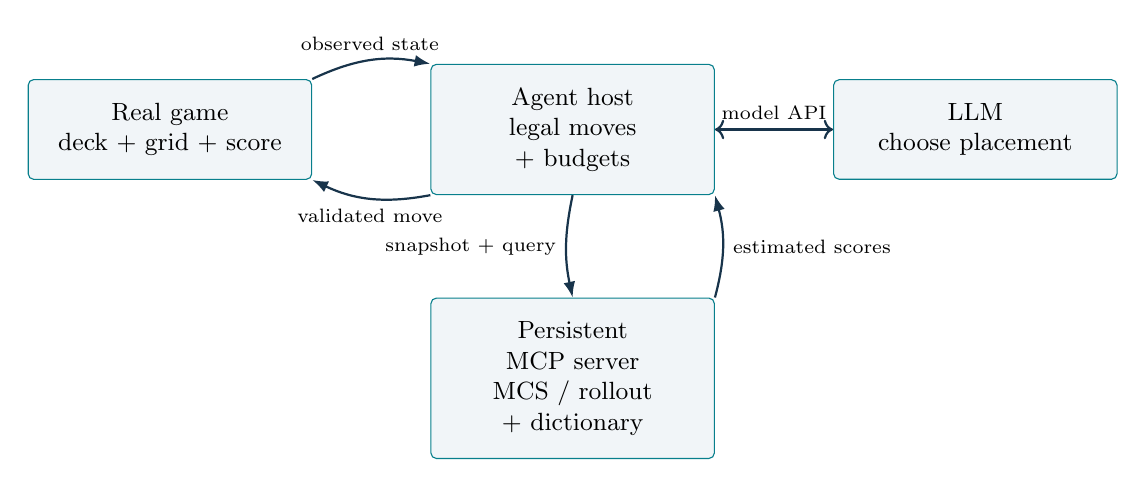
\begin{tikzpicture}[node distance=13mm and 15mm]
\node[box] (game) {Real game\\deck + grid + score};
\node[box,right=of game] (host) {Agent host\\legal moves + budgets};
\node[box,right=of host] (llm) {LLM\\choose placement};
\node[box,below=of host] (search) {Persistent MCP server\\MCS / rollout + dictionary};
\draw[arr] (game.north east) to[bend left=18] node[above,font=\scriptsize]{observed state}(host.north west);
\draw[arr] (host.south west) to[bend left=18] node[below,font=\scriptsize]{validated move}(game.south east);
\draw[<->,thick,draw=navy] (host)--node[above,font=\scriptsize]{model API}(llm);
\draw[arr] (host.south) to[bend right=12] node[left,font=\scriptsize]{snapshot + query}(search.north);
\draw[arr] (search.north east) to[bend right=15] node[right,font=\scriptsize]{estimated scores}(host.south east);
\end{tikzpicture}

\par\vspace{3mm}\raggedright\small
The host supplies the current game state. Search returns advice; the LLM selects
an index; the host validates and applies the move. The search server never
mutates the real board.
\end{frame}

\begin{frame}{Reuse resources; enforce limits}
\begin{itemize}
\item One HTTP client and one MCP process per game.
\item Discover tools and configure the dictionary once; update each position.
\item Expose only selected search tools to the model.
\item Cap rollouts and calls; reject illegal moves with bounded corrections.
\end{itemize}
\takeaway{Host-only \texttt{configure} and \texttt{set\_position} are never offered to the LLM.}
\src{src/game_agent/griddle/llm_agent.py : game_session, _choose, _decision_loop}
\small A fresh model conversation is used for each placement; process persistence
is not conversation memory.
\end{frame}

\begin{frame}{Evaluate the whole policy}
\begin{itemize}
\item Use the same deal seeds; record model, prompt, provider and search budget.
\item Compare random, standalone search, LLM alone and LLM + search.
\item Measure score, time, tokens, invalid moves and actual tool use.
\item Preserve full traces: did the LLM follow or override the advice?
\end{itemize}
\takeaway{Tool access, tool use and useful tool use are different questions.}
\small Fixed deals do not guarantee deterministic hosted model responses.
Three games are a demonstration, not a robust model ranking.
\end{frame}

\begin{frame}{Small experiment: search makes the difference}
\centering
\begin{tabular}{lrr}
\toprule Policy & Mean score & Seconds/game\\\midrule
Random & 27.3 & $<0.01$\\
Standalone MCS-10 & 84.7 & 0.60\\
Standalone MCS-200 & 93.7 & 11.88\\
GPT-4o-mini, no tools & 25.3 & 23.30\\
GPT-4o-mini + persistent MCP MCS-10 & 86.3 & 44.49\\
GPT-4.1, no tools & 24.7 & 34.92\\
GPT-4.1 + persistent MCP MCS-10 & 67.7 & 54.60\\\bottomrule
\end{tabular}
\par\vspace{3mm}\raggedright\small
Three deals (0--2), OpenRouter, original rules prompt. Standalone and tool search
use different simulation seeds. GPT-4o-mini followed all 72 search recommendations:
this shows useful delegation, not an advantage over standalone search.
\src{Completed three-deal runs; full reports and caveats: docs/griddle_llm.md.}
\end{frame}

\begin{frame}{Latency: measure before blaming the tool}
\begin{columns}[T]
\column{.46\textwidth}
\textbf{Same moves and scores}
\par\vspace{3mm}
Recreated each move: \textbf{57.73 s/game}
\par\vspace{3mm}
Reused for each game: \textbf{44.49 s/game}
\par\vspace{3mm}
Observed reduction: \textbf{22.9\%}
\column{.49\textwidth}
\textbf{Persistent run: mean seconds/game}
\par\vspace{3mm}
\begin{tabular}{lr}
LLM requests & 42.68\\
Search computation & 1.02\\
MCP startup/discovery & 0.46\\
\end{tabular}
\end{columns}
\takeaway{Most elapsed time was in model requests, not Monte Carlo search.}
\small Provider latency varies. This rerun changed both HTTP and MCP lifetime;
the timings do not isolate their separate contributions.
\src{results/griddle/llm_persistence_summary.json}
\end{frame}

\begin{frame}{PCG objective: lengthen the shortest route}
\begin{itemize}
\item A binary grid has open passages and walls; start is top-left, goal bottom-right.
\item Breadth-first search supplies exact fitness: the shortest valid route's length.
\item Mutation flips cells; a $(1+1)$ evolutionary loop retains non-worsening candidates.
\end{itemize}
\centering
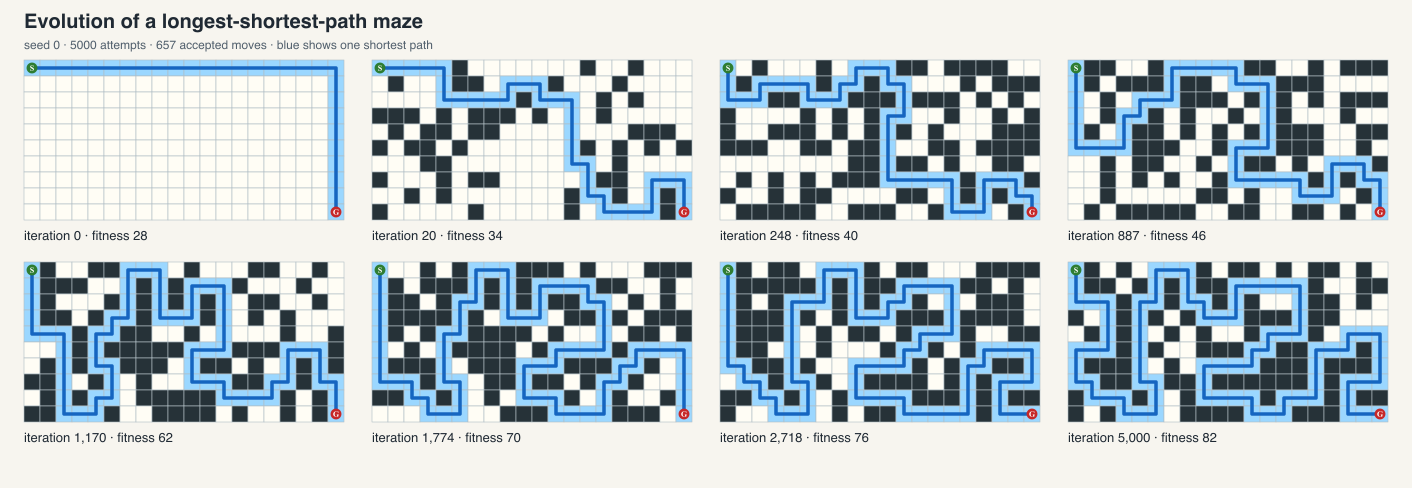
\includegraphics[width=.92\textwidth]{images/maze_evolution.png}
\par\vspace{1mm}\raggedright\scriptsize
One 20$\times$10 run, sampled across 5,000 mutation attempts; blue marks a shortest route.
\src{results/pcg/maze_evolution.svg}
\end{frame}

\begin{frame}{Maze fitness has a scale}
\centering
\begin{tabular}{lrrrr}
\toprule Grid & Iterations & Scores (seeds 0--2) & Mean & Seconds/maze\\\midrule
12$\times$8 & 2,000 & 38, 38, 38 & 38.0 & 0.09\\
12$\times$8 & 5,000 & 42, 48, 48 & 46.0 & 0.20\\
20$\times$10 & 2,000 & 70, 70, 66 & 68.7 & 0.17\\
20$\times$10 & 5,000 & 82, 88, 86 & 85.3 & 0.41\\\bottomrule
\end{tabular}
\takeaway{Compare raw path-length fitness only at the same grid dimensions.}
\small The interactive configuration was 20$\times$10 with 5,000 iterations;
the compact LLM benchmark uses 12$\times$8 with 2,000. This accounts for
scores near 80 versus 38. Times are local three-run means.
\src{Reproduced seeds 0--2; method and commands: docs/pcg_maze.md.}
\end{frame}

\begin{frame}{One-shot generation: fast evolution, diverse LLM output}
\begin{columns}[T]
\column{.46\textwidth}
\centering
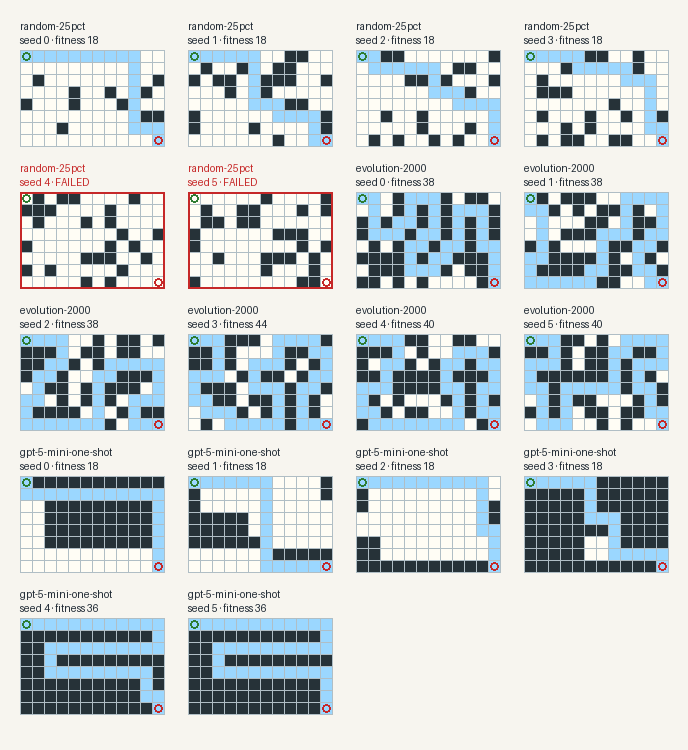
\includegraphics[height=.67\textheight]{images/maze_gpt5_mini.png}
\column{.51\textwidth}
\small
\begin{tabular}{lrrr}
\toprule Approach & Valid & Fitness & s/maze\\\midrule
Random & 4/6 & 18.0 & $<0.01$\\
Evolution-2000 & 6/6 & 39.7 & 0.08\\
GPT-5-mini & 6/6 & 24.0 & 40.65\\\bottomrule
\end{tabular}
\par\vspace{3mm}
\textbf{Set-level diversity}
\begin{itemize}
\item Mean pairwise Hamming distance: random .304, evolution .463, LLM .506.
\item Gzip size: 117, 186 and 104 bytes. Compression also reflects repeated text structure, so report both measures.
\end{itemize}
\end{columns}
\src{Six 12x8 mazes per approach: results/pcg/maze_gpt5_mini_comparison.json.}
\end{frame}

\begin{frame}{Agentic PCG: give the model a maze workshop}
\centering\resizebox{.62\textwidth}{!}{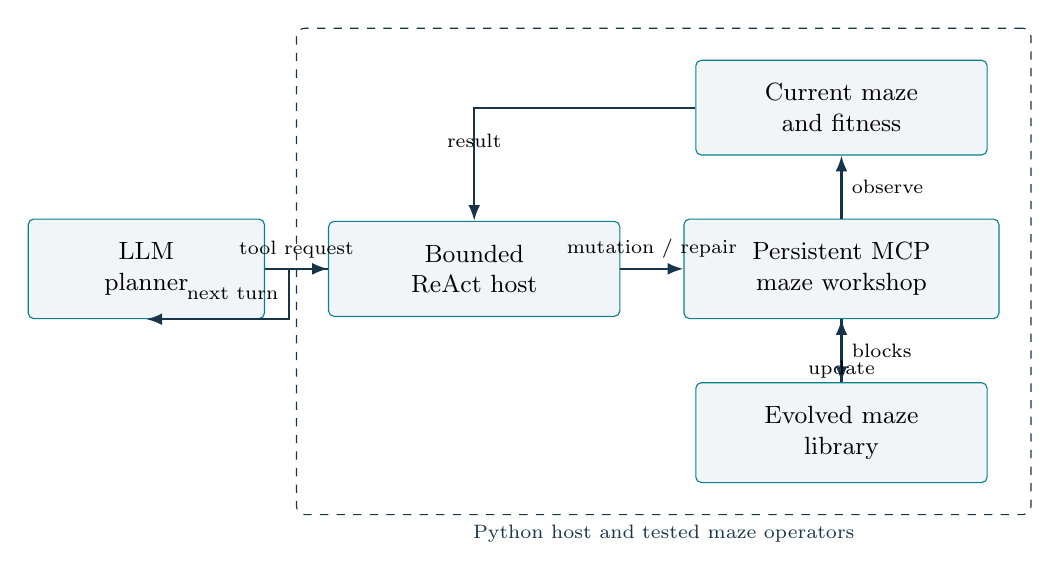
\begin{tikzpicture}[node distance=8mm and 8mm]
\node[box,text width=24mm] (llm) {LLM\\planner};
\node[box,text width=31mm,right=of llm] (host) {Bounded\\ReAct host};
\node[box,text width=34mm,right=of host] (mcp) {Persistent MCP\\maze workshop};
\node[box,text width=31mm,below=of mcp] (library) {Evolved maze\\library};
\node[box,text width=31mm,above=of mcp] (state) {Current maze\\and fitness};

\draw[arr] (llm) -- node[above,font=\scriptsize]{tool request} (host);
\draw[arr] (host) -- node[above,font=\scriptsize]{mutation / repair} (mcp);
\draw[arr] (mcp) -- node[right,font=\scriptsize]{observe} (state);
\draw[arr] (state.west) -| node[pos=.72,above,font=\scriptsize]{result} (host.north);
\draw[arr] (library) -- node[right,font=\scriptsize]{blocks} (mcp);
\draw[arr] (mcp) -- node[below,font=\scriptsize]{update} (library);
\draw[arr] (host.west) -- ++(-5mm,0) |- node[pos=.25,left,font=\scriptsize]{next turn} (llm.south);

\node[draw=navy,dashed,rounded corners=3pt,fit=(host)(mcp)(library)(state),
 inner sep=4mm,label={[font=\scriptsize,navy]below:Python host and tested maze operators}] {};
\end{tikzpicture}
}
\par\raggedright\small
\begin{itemize}\setlength\itemsep{1mm}
\item Inspect fitness and validity; request batches of local mutations.
\item Copy rectangular macro-patterns from an evolved maze library.
\item Repair disconnected candidates, then select or restore earlier states.
\end{itemize}
\par\vspace{1mm}\textbf{Tools turn generation into an observable edit--evaluate--repair loop.}
\end{frame}

\begin{frame}{Agentic maze result: validity recovered}
\begin{columns}[T]
\column{.43\textwidth}
\centering
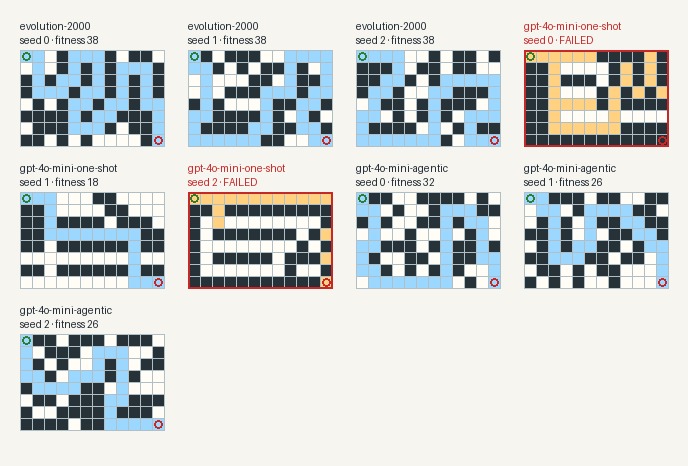
\includegraphics[width=\textwidth]{images/maze_agentic.png}
\column{.50\textwidth}
\small
\resizebox{\textwidth}{!}{%
\begin{tabular}{lrrr}
\toprule Approach & Valid & Fitness & s/maze\\\midrule
Evolution-2000 & 3/3 & 38 & 0.10\\
GPT-4o-mini one-shot & 1/3 & 18 & 1.00\\
GPT-4o-mini agentic & 3/3 & 28 & 8.97\\\bottomrule
\end{tabular}}
\par\vspace{3mm}
The agentic run made 28 model calls and 24 successful tool calls through one
persistent MCP process. Its mean pairwise Hamming distance was .479.
\par\vspace{3mm}
\textbf{Compute caveat:} each agentic maze first builds a six-member library
with 400 evolutionary iterations each. It is not an equal-compute comparison
with the 2,000-iteration baseline.
\end{columns}
\src{Three 12x8 mazes: results/pcg/maze_agentic_comparison.*}
\end{frame}

\begin{frame}[fragile]{Try it, then change one thing}
\begin{lstlisting}[language=bash,basicstyle=\ttfamily\footnotesize]
# From the repository root: no model credentials needed
uv run python src/simple_examples/direct_python.py
uv run python src/simple_examples/mcp_client.py

# Paired LLM evaluation; uses the ignored root .env
./scripts/compare_griddle_llm.sh
\end{lstlisting}
\begin{enumerate}
\item Inspect one tool request and its returned observation.
\item Change the model, prompt or rollout budget in a copied config.
\item Compare saved scores, time and tool decisions on the same deals.
\end{enumerate}
\small Hosted evaluations incur API charges. See \texttt{docs/griddle\_llm.md} for providers and configuration.
\end{frame}

\begin{frame}{Reading and code map}
\small
\begin{itemize}
\item Yao et al. (ICLR 2023), \href{https://arxiv.org/abs/2210.03629}{\textbf{ReAct: Synergizing Reasoning and Acting in Language Models}}.
\item \href{https://modelcontextprotocol.io/specification/2025-06-18/architecture}{\textbf{MCP architecture}, specification 2025-06-18}. This deck describes the repository's stdio implementation.
\item \texttt{src/simple\_examples/}: functions, server, MCP client, model loop.
\item \texttt{src/game\_agent/griddle/}: game, search server, LLM agent, benchmark.
\item \texttt{docs/griddle\_llm.md}: prompts, experiments and full report links.
\item \texttt{src/pcg/maze/}: evolution, LLM and agentic generation; visualisation.
\item \texttt{docs/pcg\_maze*.md}: PCG commands, metrics and experiment reports.
\end{itemize}
\takeaway{Build a useful tool. Connect a bounded loop. Measure the resulting behaviour.}
\end{frame}
\end{document}
